\documentclass[a4paper,12pt]{article}
\usepackage[utf8]{inputenc}
\usepackage[italian]{babel}
\usepackage{titlesec}
\usepackage{xcolor}
\usepackage{tocloft}
\usepackage{graphicx}
\usepackage{tabularx}    % Per creare tabelle con larghezza personalizzata
\usepackage[table,xcdraw]{xcolor} % Per aggiungere colori nella tabella
\usepackage{hyperref} %lo usiamo per poter inserire i link cliccabili nel documento





% Margini e formattazione
\usepackage[margin=2.5cm]{geometry}
\renewcommand{\cftsecfont}{\bfseries}
\renewcommand{\cftsecpagefont}{\bfseries}
\renewcommand{\cftsecleader}{\cftdotfill{\cftdotsep}}

% Colori per il titolo e le sezioni
\definecolor{titlecolor}{RGB}{30,144,255}
\definecolor{subtitlecolor}{RGB}{220,20,60}

% Header 
\usepackage{fancyhdr}
\pagestyle{fancy}
\fancyhf{}
\fancyhead[L]{
\includegraphics[height=1.2cm]{logo.jpg}}
\fancyhead[C]{\footnotesize Laurea Triennale in Informatica - Università di Salerno\\
Corso di Fondamenti di Intelligenza Artificiale -- Professore  F. Palomba}
\fancyfoot[C]{\thepage}

% Formattazione dei titoli
\titleformat{\section}
  {\large\bfseries\color{titlecolor}}{\thesection}{1em}{}
\titleformat{\subsection}
  {\normalsize\bfseries\color{subtitlecolor}}{\thesubsection}{1em}{}

\begin{document}

% Logo e titolo
\begin{center}
    
\includegraphics[width=0.2\textwidth]{logo.jpg}\\[0.5cm]
    \textbf{\large Laurea Triennale in Informatica - Università di Salerno}\\
    \textbf{\large Corso di Fondamenti di Intelligenza Artificiale}\\
    \textbf{\large Professore F. Palomba}\\[1.5cm]
    \textcolor{titlecolor}{\Huge }
\end{center}

\vspace{-2cm}

% Sommario Impostazioni
\setcounter{tocdepth}{3}
\renewcommand{\contentsname}{\textcolor{blue}{Sommario}}
\tableofcontents

\newpage

% Lista di tutte le voci del progetto
\section{Introduzione: sistema attuale e sistema proposto}
Oggi, con il cambiamento dello stile di vita delle persone, che preferiscono sempre più restare a casa, e a seguito della pandemia, le piattaforme di streaming hanno ottenuto un successo crescente. Già ampiamente utilizzate, queste piattaforme permettono di guardare film e serie TV su qualsiasi dispositivo connesso a Internet. Con l’aumento della loro popolarità, hanno sentito l’esigenza di rendere l’esperienza dell’utente sempre più personalizzata, introducendo nuove funzionalità.\\
Inizialmente, i problemi principali erano due: da un lato, l’utente accedeva alla piattaforma sapendo già cosa guardare, limitandosi semplicemente a visualizzare i contenuti scelti per poi uscire; dall’altro lato, numerosi utenti, incerti su cosa guardare, si trovavano disorientati dalla vasta offerta disponibile e, di conseguenza, spesso abbandonavano l’idea di selezionare un contenuto.\\
A partire dal 2006, con l’introduzione dei primi algoritmi di raccomandazione su Netflix, è iniziata una trasformazione che ha rivoluzionato il modo in cui gli utenti fruiscono dei contenuti. Inizialmente, questi algoritmi si limitavano a proporre i contenuti più popolari, più visti e le ultime uscite. Successivamente, si sono evoluti, ponendo l’utente al centro dell’esperienza. Oggi, i contenuti vengono consigliati sulla base delle preferenze individuali, tenendo conto non solo dei contenuti già visti e dei generi preferiti, ma anche di attori, registi e altre caratteristiche, come le case di produzione.\\
Utilizzando piattaforme di streaming come Netflix o Prime Video, si può apprezzare il progresso degli algoritmi di intelligenza artificiale, che rendono l’esperienza dell’utente ancora più immersiva e dinamica.\\
Il progetto proposto mira a realizzare una web app ottimizzata per smart TV, che consenta agli utenti di scoprire nuovi contenuti da guardare. L’app offrirà la possibilità di accedere a informazioni dettagliate sui film, inclusi trailer e indicazioni sulle piattaforme dove sono disponibili. In particolare, il sistema sfrutterà i dati derivati dalla lista di preferiti dell’utente per consigliare contenuti in linea con i suoi gusti, considerando elementi come genere, cast, produzione e anno di uscita. Il tutto sarà supportato da tecniche di intelligenza artificiale, simili a quelle già adottate dalle principali piattaforme di streaming.
Il codice completo del progetto è disponibile nella repository GitHub a questo \textcolor{blue}{\href{https://github.com/LRuocco22/NozApp/}{\textbf{{link}}}}.
\section{Descrizione dell’agente}

    \subsection{Obiettivi}
			Lo scopo del progetto è quello di realizzare un agente intelligente che sia in grado di:
	\begin{itemize}
		 \item Generare un insieme di film basandosi sulla lista dei preferiti dell'utente;
		 \item Consigliare una lista di contenuti correlati nella schermata di dettaglio del singolo film;
  		 \item Nel consigliare i film, non deve tenere conto di una singola caratteristica, ma di tutte le informazioni che possono essere utilizzate per personalizzare al meglio la lista di film.
	\end{itemize}

\newpage %Vado alla nuova pagina per far entrare tutta la tabella in una sola pagina
\subsection{Specifica PEAS}
Diamo ora la specifica PEAS dell'agente:
\begin{table}[h!]
    \centering
    \renewcommand{\arraystretch}{1.5} % Spazio tra le righe
    \setlength{\tabcolsep}{8pt} % Spazio tra colonne
    \begin{tabularx}{\textwidth}{|>{\columncolor[HTML]{CFE2F3}}l|X|}
        \hline
        \rowcolor[HTML]{CFE2F3} 
        \textbf{PEAS}              & \textbf{Descrizione}                                                                                                                                                                                                                                                                                         \\ \hline
        \textbf{Performance}       & La misura di performance dell'agente è la sua capacità di avvicinarsi quanto più possibile a una situazione ideale nella quale vengano mostrati agli utenti esattamente i film che loro desiderano guardare e ai quali sono interessati.                                                                                           				\\ \hline
        \textbf{Environment}       & L’ambiente in cui opera l’agente è lo spazio dell'utente dell'app, con le sue preferenze, unito a quello dei possibili film e le loro caratteristiche. L’ambiente è:
                            \begin{itemize}
                              \item \textbf{Dinamico}, in quanto nel corso delle elaborazioni dell’agente, l'utente aggiunge un film alla sua lista di preferiti, cambiando in tal modo le sue preferenze;
                              \item \textbf{Episodico}, le decisioni prese in un episodio non influenzano le decisioni successive;
			\item 	L'ambiente è \textbf{Discreto} perchè gli stati (film) e le azioni (suggerimenti) sono limitati e finiti, basati su attributi come genere, cast e tag, che hanno un numero definito di valori;
                              \item \textbf{Completamente osservabile}, in quanto si ha accesso a tutte le informazioni relative al catalogo di contenuti e alle preferenze dell'utente in ogni momento;
                              \item \textbf{Non deterministico}, in quanto lo stato dell’ambiente cambia indipendentemente dalle azioni dell’agente;
                              \item \textbf{Non noto}, in quanto l’agente non può conoscere a priori il risultato esatto delle sue azioni, in termini di efficienza;
                              \item \textbf{Stocastico e unico}, in quanto l’unico agente che opera in questo ambiente è quello in oggetto.
                            \end{itemize}            
                                                \\ \hline
        \textbf{Actuators}         & Gli attuatori dell’agente consistono nella lista dei film consigliati sulla base delle preferenze dell'utente e il relativo carrello che li mostra.                                                                                                                                                                                  					\\ \hline
        \textbf{Sensors}           & I sensori dell’agente consistono nella lista di film preferiti dell'utente e le informazioni sul catalogo dei film.                                                                                                                                                                                                      					\\ \hline
    \end{tabularx}
    \caption{Specifica PEAS dell'agente}
\end{table}

   \newpage
    \subsection{Analisi del problema}
	L'implementazione del modulo di raccomandazione è stata guidata dall'obiettivo di replicare i sistemi di raccomandazione esistenti, introducendo alcune differenze significative. In particolare, il focus è posto esclusivamente sui gusti del singolo utente, evitando di basarsi sui dati o sulle preferenze di altri utenti.\\ Per perseguire questa visione, si è scelto di eliminare la necessità di registrazione, rendendo l'applicazione più accessibile e immediata per l'utente finale.\\Questa scelta progettuale favorisce un'esperienza personalizzata e inclusiva, garantendo al contempo la semplicità d'uso. \\ \\
	Si è scelto di interpretare il problema come un problema di \textbf{Clustering}. L'idea è stata di analizzare la lista dei film preferiti dall'utente, estrarre le informazioni rilevanti da questi, e generare una lista di film che rispecchiassero i suoi gusti, suggerendo contenuti che potessero piacergli.

\section{Raccolta, analisi e preprocessing dei dati}

    \subsection{Scelta del dataset} 
		Andando a parlare del dataset necessario per la creazione del modello di machine learning, si potevano considerare due possibili approcci:

		\begin{enumerate}
   			 \item \textbf{Creare} un dataset da zero, raccogliendo informazioni su tutti i film, anche quelli più vecchi, e concentrandosi sugli aspetti salienti come generi e rilevanza dei vari tag;
    			 \item \textbf{Cercare} un dataset già formato e adattarlo alle specifiche esigenze del progetto.
		\end{enumerate}

		La prima soluzione risultava impraticabile, dato l'enorme numero di film presenti nella storia e la varietà di caratteristiche che sarebbe stato necessario raccogliere e inserire. Tale approccio avrebbe portato alla creazione di un dataset poco popolato e privo di molte informazioni importanti.

		Si è quindi deciso di procedere cercando in rete un dataset già esistente. Dopo aver considerato diverse opzioni, si è scelto il dataset MovieLens, che si è rivelato il più adatto alle necessità del progetto.

    \subsection{Analisi e scrematura del dataset}
Il dataset considerato, consultabile a questo \textcolor{blue}{\href{https://grouplens.org/datasets/movielens/latest/}{\textbf{{link}}}}, è stato scelto per un importante aspetto che presenta al suo interno. MovieLens assegna a ogni film uno specifico ID e si è notato che contiene anche l'ID corrispondente con cui i film sono identificati nell'API di TMDb, utilizzata nella web app dove questo modulo è inserito. Questo ha permesso al dataset di integrarsi perfettamente con l'applicazione, evitando un problema significativo: quello di dover trovare un modo per far corrispondere gli ID dei film sia quando si considerano i preferiti per la raccomandazione, sia quando si genera la lista dei film consigliati. Infatti, per visualizzare i film nell'app, è necessario fare chiamate all'API di TMDb usando gli ID di quest'ultima, e non quelli del dataset.
\newpage
        \subsubsection{Tabella Movies} 
		\begin{table}[h!]
			\centering
				\begin{tabular}{|c|l|l|}
					\hline
					\textbf{Colonna} & \textbf{Descrizione} & \textbf{Tipo di Dato} \\ \hline
					\texttt{movieId} & Identificatore univoco del film & Numerico (Intero) \\ \hline
					\texttt{title} & Titolo del film, include l'anno tra parentesi & Testo \\ \hline
					\texttt{genres} & Generi del film, separati da pipe (\texttt{|}) & Testo (lista di generi) \\ \hline
				\end{tabular}
			\caption{Descrizione delle colonne nel file \texttt{movies.csv} del dataset MovieLens.}
		\end{table}

        \subsubsection{Tabella Links}
		\begin{table}[h!]
			\centering
				\begin{tabular}{|c|l|l|}
					\hline
					\textbf{Colonna} & \textbf{Descrizione} & \textbf{Tipo di Dato} \\ \hline
					\texttt{movieId} & Identificatore univoco del film & Numerico (Intero) \\ \hline
					\texttt{imdbId} & Identificatore univoco del film su IMDb & Testo (Stringa) \\ \hline
					\texttt{tmdbId} & Identificatore univoco del film su TMDb & Numerico (Intero) \\ \hline
				\end{tabular}
			\caption{Descrizione delle colonne nel file \texttt{links.csv} del dataset MovieLens.}
		\end{table}

        \subsubsection{Tabella Genome-Scores}
			\begin{table}[h!]
				\centering
					\begin{tabular}{|c|l|l|}
						\hline
						\textbf{Colonna} & \textbf{Descrizione} & \textbf{Tipo di Dato} \\ \hline
						\texttt{movieId} & Identificatore univoco del film & Numerico (Intero) \\ \hline
						\texttt{tagId} & Identificatore univoco per un tag associato al film & Numerico (Intero) \\ \hline
						\texttt{relevance} & Livello di rilevanza del tag per il film & Numerico (Decimale) \\ \hline
					\end{tabular}
				\caption{Descrizione delle colonne nel file \texttt{genome-scores.csv} del dataset MovieLens.}
			\end{table}

        \subsubsection{Tabella Genome-Tags}
			\begin{table}[h!]
				\centering
					\begin{tabular}{|c|l|l|}
						\hline
						\textbf{Colonna} & \textbf{Descrizione} & \textbf{Tipo di Dato} \\ \hline
						\texttt{tagId} & Identificatore univoco per ogni tag & Numerico (Intero) \\ \hline
						\texttt{tag} & Etichetta associata ad ogni film & Testo(Stringa) \\ \hline
					\end{tabular}
				\caption{Descrizione delle colonne nel file \texttt{genome-tags.csv} del dataset MovieLens.}
			\end{table}

\newpage

        \subsubsection{Tabella Ratings}
			\begin{table}[h!]
				\centering
					\begin{tabular}{|c|l|l|}
						\hline
						\textbf{Colonna} & \textbf{Descrizione} & \textbf{Tipo di Dato} \\ \hline
						\texttt{userId} & Identificatore univoco dell'utente & Numerico (Intero) \\ \hline
						\texttt{movieId} & Identificatore univoco del film & Numerico (Intero) \\ \hline
						\texttt{rating} & Valutazione del film da parte dell'utente (0.5-5) & Numerico (Decimale) \\ \hline
						\texttt{timestamp} & Data e ora della valutazione & Data/Ora (Timestamp) \\ \hline
					\end{tabular}
				\caption{Descrizione delle colonne nel file \texttt{ratings.csv} del dataset MovieLens.}
			\end{table}

        \subsubsection{Tabella Tags}
			\begin{table}[h!]
				\centering
					\begin{tabular}{|c|l|l|}
						\hline
						\textbf{Colonna} & \textbf{Descrizione} & \textbf{Tipo di Dato} \\ \hline
						\texttt{userId} & Identificatore univoco dell'utente & Numerico (Intero) \\ \hline
						\texttt{movieId} & Identificatore univoco del film & Numerico (Intero) \\ \hline
						\texttt{tag} & Etichetta o tag associato al film & Testo (Stringa) \\ \hline
						\texttt{timestamp} & Data e ora in cui è stato assegnato il tag & Data/Ora (Timestamp) \\ \hline
					\end{tabular}
				\caption{Descrizione delle colonne nel file \texttt{tags.csv} del dataset MovieLens.}
			\end{table}


    \subsection{Preprocessing dei Dati}
	In questa fase viene fatto il preprocessing dei dati cinematografici e del loro clustering utilizzando tecniche di machine learning.\\Lo scopo è creare un dataset arricchito e organizzare i film in gruppi significativi basati sui generi e sui tag di rilevanza. Di seguito, vengono illustrate in dettaglio tutte le fasi implementate, con riferimenti al codice specifico.
        \subsubsection{Caricamento dei dati}
	Nella prima fase, i dati provenienti da più file CSV vengono caricati utilizzando la libreria "pandas". 
\begin{verbatim}
# Percorsi dei file
movies_path = '../movielens/movies.csv'
links_path = '../movielens/links.csv'
genome_scores_path = '../movielens/genome-scores.csv'
genome_tags_path = '../movielens/genome-tags.csv'

# Step 1: Caricamento dei file
movies_df = pd.read_csv(movies_path)
links_df = pd.read_csv(links_path).drop(columns=['imdbId'])
genome_scores_df = pd.read_csv(genome_scores_path)
genome_tags_df = pd.read_csv(genome_tags_path)
\end{verbatim}

	Il risultato è la creazione di strutture dati tabulari(DataFrame) per ogni file, che saranno utilizzate nelle fasi successive. 
	Questa fase è essenziale per acquisire i dati necessari per l'elaborazione successiva, garantendo una struttura coesa per l'integrazione e l'analisi.
	\subsubsection{Pulizia dei Dati}
	In questa fase vengono eliminate tutte le informazioni che non concorrono al corretto funzionamento del modulo di raccomandazione.\\
	Di seguito il codice dove vengono effettuate tali operazioni:
	\begin{itemize}
		\item{Rimozione dei film che non possiedono il \textbf{tmdbID}: }
\begin{verbatim}
links_df = links_df[links_df['tmdbId'].notnull()&(links_df['tmdbId'] > 0)] 
\end{verbatim}
I film che non dispongono di un identificativo TMDb (tmdbID) vengono esclusi, poiché l'applicazione effettua chiamate all'API di TMDb per recuperare informazioni aggiuntive. L'assenza di questo identificativo impedirebbe la corretta visualizzazione dei dettagli del film.
		\item{Rimozione dei film con \textbf{('no genres listed')}:}
\begin{verbatim}
movies_df = movies_df[movies_df['genres'] != '(no genres listed)']
\end{verbatim}
I film il cui campo genres contiene il valore "(no genres listed)" vengono scartati.\\La mancanza di informazioni sui generi potrebbe compromettere l'accuratezza delle raccomandazioni, che si basano sui gusti degli utenti e sulle caratteristiche dei film.
		\item{Rimozione della colonna \textbf{imdbID}:}
\begin{verbatim}
links_df = links_df.drop(columns=['imdbId'])
\end{verbatim}
La colonna imdbID viene rimossa, in quanto non è necessaria per le funzionalità previste dal progetto e non viene utilizzata dal modulo di raccomandazione.

\end{itemize}
        \subsubsection{Unione dei Dataset}
	\label{sec:unione-dataset}
	Questa fase del processo si occupa di combinare i dati provenienti da diversi file per costruire un dataset unificato.
	L'obiettivo è quello di integrare i dati relativi ai film, ai tag di rilevanza e ai collegamenti con altre risorse per creare una rappresentazione coerente e che supporti le analisi successive. Questa fase prevede tre passaggi fondamentali:
			\begin{enumerate}
   			 \item \textbf{Unione tra "genome-scores" e "genome-tags"} \\
				Le informazioni sui punteggi di rilevanza sono uniti ai rispettivi nomi dei tag utilizzando la colonna "tagId".

\begin{verbatim}
genome_scores_with_tags = genome_scores_df.merge(genome_tags_df, on="tagId")
\end{verbatim}

    			 \item \textbf{Integrazione con il dataset dei film} \\
				La tabella "movies.csv", contenente titoli e generi dei film, è arricchita con i tag e i relativi punteggi di rilevanza, sfruttando la colonna "movieId" come chiave comune.
\begin{verbatim}
movies_with_tags = movies_df.merge(genome_scores_with_tags, on="movieId")
\end{verbatim}

			 \item \textbf{Aggiunta dei collegamenti a TMDb}\\
				Vengono aggiunte le informazioni provenienti da "links.csv"(colonna tmdbId), per associare ogni film a una risorsa esterna  (es. TMDb).
				
\begin{verbatim}
final_dataset = 
				movies_with_tags.merge(links_df[['movieId', 'tmdbId']],on="movieId")
\end{verbatim}
			\item \textbf{Eliminazione di tutti i film senza tag: }
				Infine, si procede eliminando i film senza tag. Questo passaggio è molto importante in quanto considerandoli si otterrebbero delle raccomandazioni poco accurate.
\begin{verbatim}
tagged_movie_ids = genome_scores_with_tags['movieId'].unique()
movies_df = movies_df[movies_df['movieId'].isin(tagged_movie_ids)]
\end{verbatim}

		\end{enumerate}

	Il risultato di questa fase è un dataset unificato, che combina i dati principali dei film con i dettagli relativi ai generi, ai tag e ai collegamenti esterni.

        \subsubsection{Preprocessing per il Clustering}
		Questa fase è cruciale per preparare i dati grezzi in una forma che consenta di applicare efficacemente tecniche di clustering. In questa parte vengono integrate informazioni dui generi e sui punteggi di rilevanza dei tag, trasformandole in una matrice delle feature. Si vuole quindi creare una rappresentazione vettoriale coerente dei film, che combini generi e rilevanza dei tag, pronta per l'algoritmo di clustering. Vengono eseguiti tre passaggi chiave: 

			\begin{enumerate}
   			 \item \textbf{Codifica dei generi cinematografici} \\
				I generi dei film, originariamente rappresentati come stringhe separate da pipe,  vengono convertiti in una lista e successivamente codificati in variabili binarie utilizzando "MultiLabelBinarizer". Il risultato è un DataFrame (genres-encoded) che associa a ciascun "movieId" un vettore binario rappresentante i generi.
						%\includegraphics[]{./ScreenScript/1.png}
\begin{verbatim}
movies_df['genres_list'] = movies_df['genres'].apply(lambda x: x.split('|'))
mlb = MultiLabelBinarizer()
genres_encoded = pd.DataFrame(mlb.fit_transform(movies_df['genres_list']),
                 columns=mlb.classes_, index=movies_df['movieId'])
\end{verbatim}

    			 \item \textbf{Calcolo dei punteggi medi di rilevanza per tag} \\
						Si utilizza il dataset unificato generato nella fase \hyperref[sec:unione-dataset]{\textbf{Unione dei Dataset}}  per aggregare i punteggi di rilevanza delle tag per ogni film. Questo consente di ottenere una rappresentazione compatta dei punteggi medi per ogni tag. Si ottiene, quindi, un DataFrame (tag-relevance) in cui: le righe rappresentano i film (movieId), le colonne i tag, e i valori indicano il punteggio medio di rilevanza del tag per quel film.
\begin{verbatim}
tag_relevance = final_dataset.groupby(['movieId', 'tag'])['relevance']
		              .mean().unstack(fill_value=0)
\end{verbatim}
					%\begin{center}
						%\includegraphics[]{./ScreenScript/2.png}
					%\end{center}
\newpage
			 \item \textbf{Creazione della matrice delle feature}\\
				I dati codificati dei generi e i punteggi delle tag vengono uniti per creare una matrice completa, in cui ogni film è rappresentato da un vettore di caratteristiche numeriche. I passaggi effettuati sono: 
							\begin{itemize}
								\item \textbf{Concatenazione: } le due componenti (genres-encoded e tag-relevance) vengono unite lungo le colonne.
								\item \textbf{Gestione dei valori mancanti: } le posizioni vuote vengono riempite con il valore "0" utilizzando "fillna(0)".
								\item \textbf{Filtraggio degli indici: } Si assicura che i film presenti nella matrice abbiano corripondenza nei dati originali (movies-df).
							\end{itemize}

						%\begin{center}
						% \includegraphics[]{./ScreenScript/3.png}
						%\end{center}
\begin{verbatim}
feature_matrix = 
			pd.concat([genres_encoded, tag_relevance], axis=1, sort=False).fillna(0)
feature_matrix = 
			feature_matrix.loc[feature_matrix.index.intersection(movies_df['movieId'])]
\end{verbatim}
					Il risultato finale di questa fase è la matrice delle feature (feature-matrix), che rappresenta la base per il clustering. Questa matrice fornisce una descrizione numerica completa e scalabile di ogni film, combinando, generi codificati come variabili binarie e rilevanza media delle tag. Questa rappresentazione garantisce che ogni film sia rappresentato in uno spazio vettoriale uniforme, rendendolo idoneo per l'algoritmo \textbf{KMeans} nella fase successiva.

		\end{enumerate}

        \subsubsection{Preprocessing per il Clustering}
		Questa fase è cruciale per preparare i dati grezzi in una forma che consenta di applicare efficacemente tecniche di clustering. In questa parte vengono integrate informazioni dui generi e sui punteggi di rilevanza dei tag, trasformandole in una matrice delle feature. Si vuole quindi creare una rappresentazione vettoriale coerente dei film, che combini generi e rilevanza dei tag, pronta per l'algoritmo di clustering. Vengono eseguiti tre passaggi chiave: 

			\begin{enumerate}
   			 \item \textbf{Codifica dei generi cinematografici} \\
				I generi dei film, originariamente rappresentati come stringhe separate da pipe,  vengono convertiti in una lista e successivamente codificati in variabili binarie utilizzando "MultiLabelBinarizer". Il risultato è un DataFrame (genres-encoded) che associa a ciascun "movieId" un vettore binario rappresentante i generi.
						%\includegraphics[]{./ScreenScript/1.png}
\begin{verbatim}
movies_df['genres_list'] = movies_df['genres'].apply(lambda x: x.split('|'))
mlb = MultiLabelBinarizer()
genres_encoded = pd.DataFrame(mlb.fit_transform(movies_df['genres_list']),
                 columns=mlb.classes_, index=movies_df['movieId'])
\end{verbatim}
\newpage
    			 \item \textbf{Calcolo dei punteggi medi di rilevanza per tag} \\
						Si utilizza il dataset unificato generato nella fase \hyperref[sec:unione-dataset]{\textbf{Unione dei Dataset}}  per aggregare i punteggi di rilevanza delle tag per ogni film. Questo consente di ottenere una rappresentazione compatta dei punteggi medi per ogni tag. Si ottiene, quindi, un DataFrame (tag-relevance) in cui: le righe rappresentano i film (movieId), le colonne i tag, e i valori indicano il punteggio medio di rilevanza del tag per quel film.
\begin{verbatim}
tag_relevance = final_dataset.groupby(['movieId', 'tag'])['relevance']
		              .mean().unstack(fill_value=0)
\end{verbatim}
			 \item \textbf{Creazione della matrice delle feature}\\
				I dati codificati dei generi e i punteggi delle tag vengono uniti per creare una matrice completa, in cui ogni film è rappresentato da un vettore di caratteristiche numeriche. I passaggi effettuati sono: 
							\begin{itemize}
								\item \textbf{Concatenazione: } le due componenti (genres-encoded e tag-relevance) vengono unite lungo le colonne.
								\item \textbf{Gestione dei valori mancanti: } le posizioni vuote vengono riempite con il valore "0" utilizzando "fillna(0)".
								\item \textbf{Filtraggio degli indici: } Si assicura che i film presenti nella matrice abbiano corripondenza nei dati originali (movies-df).
							\end{itemize}

						%\begin{center}
						% \includegraphics[]{./ScreenScript/3.png}
						%\end{center}
\begin{verbatim}
feature_matrix = 
			pd.concat([genres_encoded, tag_relevance], axis=1, sort=False).fillna(0)
feature_matrix = 
			feature_matrix.loc[feature_matrix.index.intersection(movies_df['movieId'])]
\end{verbatim}
					Il risultato finale di questa fase è la matrice delle feature (feature-matrix), che rappresenta la base per il clustering. Questa matrice fornisce una descrizione numerica completa e scalabile di ogni film, combinando, generi codificati come variabili binarie e rilevanza media delle tag. Questa rappresentazione garantisce che ogni film sia rappresentato in uno spazio vettoriale uniforme, rendendolo idoneo per l'algoritmo \textbf{KMeans} nella fase successiva.

		\end{enumerate}
\newpage
\section{Algoritmo di clustering}
    \subsection{Scelta dell’algoritmo di clustering}
L'approccio basato sul clustering è stato scelto per affrontare il problema della raccomandazione di film in quanto consente di raggruppare i film in base a caratteristiche condivise, come generi e tag, senza la necessità di conoscere a priori le preferenze specifiche di un utente. Questa segmentazione permette di identificare gruppi omogenei di film, migliorando l'efficienza del sistema di raccomandazione: una volta identificato il cluster di appartenenza di un film preferito dall’utente, si possono suggerire altri film dello stesso gruppo, riducendo la complessità computazionale rispetto a confronti diretti con l’intero dataset.
        \subsubsection{K-Means}
	L'algoritmo K-Means è stato selezionato come metodo di clustering per le seguenti ragioni:
	\begin{enumerate}
		\item \textbf{Efficienza su grandi dataset: }K-Means è un algoritmo iterativo e scalabile che lavora in tempo lineare rispetto al numero di punti dati, risultando ideale per dataset di grandi dimensioni come MovieLens.
		\item \textbf{Capacità di gestire feature multidimensionali: }Nel preprocessing, i dati categoriali (generi) e continui (punteggi di rilevanza dei tag) vengono combinati in una matrice di feature numeriche. K-Means è particolarmente adatto per individuare cluster in uno spazio multidimensionale come questo.
		\item \textbf{Interpretabilità dei cluster: }I risultati di K-Means sono facilmente interpretabili, poiché ogni film viene assegnato a un cluster specifico basato sulla prossimità nello spazio delle feature. Questo facilita l’analisi e l’utilizzo pratico per generare raccomandazioni.
		\item \textbf{Flessibilità nella scelta del numero di cluster: }K-Means consente di ottimizzare il valore di \textbf{K} in base alle caratteristiche del dataset
\newpage
		\item \textbf{Distribuzione dei Dati: }
La scelta di K-Means è stata rafforzata dall'analisi preliminare della distribuzione dei dati, rappresentata attraverso un grafico generato con la PCA. Questo grafico, che proietta i dati in uno spazio bidimensionale, evidenzia una distribuzione densa e compatta, come mostrato di seguito:

\begin{center}
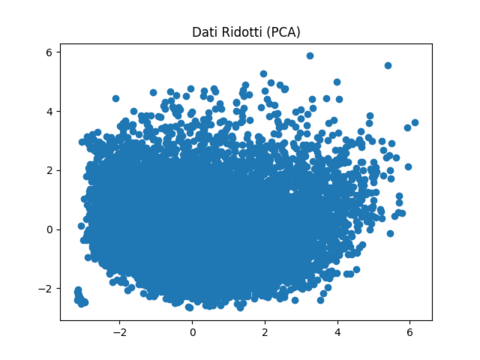
\includegraphics[]{D:/ProgettoFIA/DocumentazioneProgetto/DocumentazioneLaTex/ScreenScript/PCA.png}

\textit{Figura 1: Distribuzione dei dati rappresentata con PCA.}
\end{center}

La compattezza della distribuzione suggerisce che i dati sono ben raggruppati e privi di dispersioni significative, un aspetto cruciale per l'efficacia di K-Means. Questa struttura consente all'algoritmo di identificare i cluster con maggiore precisione, riducendo l'impatto di eventuali outlier e garantendo una convergenza stabile dei centroidi. Inoltre, l'assenza di separazioni complesse o sovrapposizioni significative tra i dati rende la distanza euclidea, su cui si basa K-Means, una metrica adatta per il clustering in questo contesto.
	\end{enumerate}
\newpage
	\subsubsection{Scelta del numero di Cluster}
La selezione del numero di cluster \textbf{K = 4} è stata effettuata attraverso un'analisi rigorosa basata su metriche quantitative e considerazioni pratiche, per garantire un compromesso ottimale tra la coerenza interna dei cluster, la separazione tra gruppi distinti e l'utilità del modello per il progetto.
		\begin{itemize}
			\item \textbf{Elbow Point Method} : 
				\begin{center}
					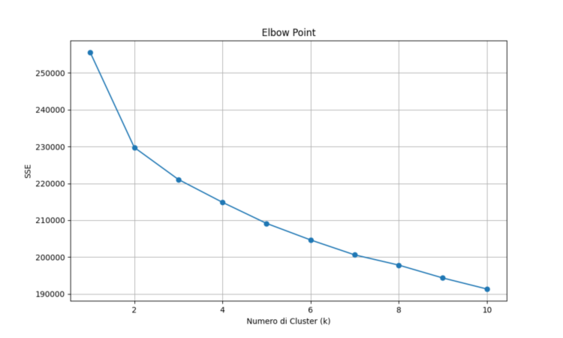
\includegraphics[]{D:/ProgettoFIA/DocumentazioneProgetto/DocumentazioneLaTex/ScreenScript/elbow_point.png}

\textit{Figura 2: Metodo Elbow per identificare il numero ottimale di cluster.}
				\end{center}


Dal grafico della somma degli errori al quadrato (SSE), si osserva un gomito più evidente per \textbf{K = 2}, che indica una significativa riduzione dell'errore intra-cluster rispetto a un solo cluster. Tuttavia, la riduzione continua per valori più alti di \textbf{K}, con un rallentamento evidente a partire da \textbf{K = 4}. Questa evidenza suggerisce che \textbf{K = 4} rappresenta un compromesso tra semplicità e capacità del modello di catturare la struttura dei dati.

\newpage
			\item \textbf{Valutazione tramite il Silhouette Score: } Il Silhouette Score misura la qualità del clustering considerando sia la coesione interna (quanto i punti sono vicini al centro del loro cluster) sia la separazione tra cluster.

	\begin{center}
		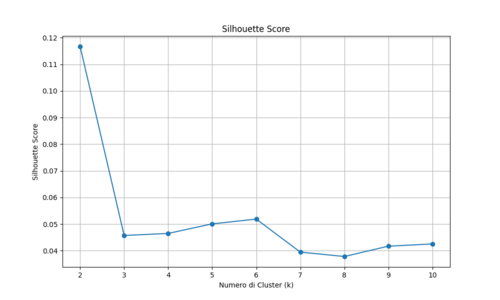
\includegraphics[]{D:/ProgettoFIA/DocumentazioneProgetto/DocumentazioneLaTex/ScreenScript/silhouette_score.png}

\textit{Figura 3: Analisi del punteggio Silhouette per valutare la coesione e la separazione dei cluster.}
	\end{center}


Il valore massimo del Silhouette Score si osserva per \textbf{K = 2}, il che indica che i cluster sono ben separati e coesi a questo livello. Tuttavia, scegliere \textbf{K = 2} produrrebbe una segmentazione eccessivamente generica, con solo due grandi gruppi, che non rifletterebbero adeguatamente la complessità e la varietà dei dati. Per \textbf{K = 4}, il punteggio rimane accettabile, garantendo comunque una buona separazione tra i cluster, ma consentendo una segmentazione più dettagliata e significativa.
		\end{itemize}


La scelta di \textbf{K = 4} rappresenta un equilibrio ideale tra la semplicità suggerita dai grafici (\textbf{K = 2}) e la necessità di una segmentazione più significativa per il progetto. Questo valore consente di catturare la diversità delle caratteristiche dei dati senza introdurre complessità inutili, offrendo una soluzione più dettagliata e utile per il sistema di raccomandazione.
\newpage
\subsubsection{Implementazione dell'algoritmo KMeans}
Lo script seguente implementa l'algoritmo K-Means per segmentare i film del dataset MovieLens in base ai loro generi e tag.
L'obiettivo è identificare gruppi di film con caratteristiche simili per supportare un sistema di raccomandazione efficiente e scalabile. Di seguito viene descritto il processo in dettaglio.
\begin{center}
\begin{verbatim}
# Step 5: Clustering con KMeans
num_clusters = 4
kmeans = KMeans(n_clusters=num_clusters, random_state=42)
clusters = kmeans.fit_predict(feature_matrix)

# Salva i centroidi dei cluster
centroids = kmeans.cluster_centers_
pd.DataFrame(centroids).to_csv('kmeans_cluster_centers.csv',index=False,header=False)

# Associare i cluster ai film
movies_with_clusters = movies_df.set_index('movieId')
				.join(links_df.set_index('movieId'), how='inner')
movies_with_clusters['cluster'] = pd.Series(clusters, index=feature_matrix.index)

# Step 6: Salvataggio dei risultati
movies_with_clusters.reset_index().to_csv('movies_with_clusters.csv', index=False)
feature_matrix.to_csv('feature_matrix.csv', index=True)

print("Clustering completato. I risultati sono stati salvati.")
\end{verbatim}
\end{center}
L'implementazione di K-Means nel sistema di raccomandazione inizia con la definizione del numero di cluster (\textbf{K = 4}). \\Il modello viene poi inizializzato specificando \textbf{n-clusters = 4 }per definire il numero di gruppi e \textbf{random-state = 42 }per garantire che i risultati siano riproducibili.\\
Successivamente, il modello viene addestrato sulla matrice delle feature che rappresenta ogni film in uno spazio multidimensionale, dove le dimensioni corrispondono ai generi e ai tag dei film. L'algoritmo K-Means assegna quindi ciascun film a uno dei cluster in base alla vicinanza nello spazio delle feature.\\
Una volta completato il clustering, i risultati vengono associati ai film utilizzando il loro indice comune. Questo consente di arricchire il dataset originale dei film con le informazioni sul cluster di appartenenza, integrando dettagli utili per il sistema di raccomandazione.
\\I risultati finali vengono esportati in tre file separati.\\
Il primo, \textbf{kmeans-cluster-centers.csv}, è un file che contiene le coordinate dei centroidi calcolati dall'algoritmo di clustering K-Means.\\Il secondo, \textbf{movies-with-clusters.csv},  contiene i risultati del clustering con informazioni sui film.\\Il terzo, \textbf{feature-matrix.csv} è una matrice che rappresenta le caratteristiche numeriche dei film, utilizzata per il clustering, dove ogni riga rappresenta un film mentre ogni colonna una caratteristica.\\
Il processo si conclude con un messaggio di conferma che informa che il clustering è stato completato e i risultati sono stati salvati. Questo approccio assicura un'integrazione fluida del modello K-Means nel sistema, consentendo di segmentare il dataset MovieLens in modo efficace e scalabile.
\section{Integrazione con il sistema}
\subsection{Architettura e Funzionalità Principali}
\subsection{Logica Implementata: }
\subsubsection{Risposta e Error Handling}
\subsection{Logica Interna e Dettagli Tecnici}
\subsection{Implementazione dello script: }
\section{Glossario}
\end{document}





